\title{Estimating population average treatment effects from experiments with noncompliance}

\author{Kellie Ottoboni, Jason Poulos}

\date{\today}

%%%%%%%%%%%%%%%%%%%%%%%%%%%%%%%%%%%%%%%%%%%%%%%%%%
% Set document class
\documentclass[12pt]{article}

% Define packages
\usepackage{graphicx,amsfonts,psfrag,layout,subcaption,array,longtable,lscape,booktabs,dcolumn,natbib,amsmath,amssymb,amssymb,amsthm,setspace,epigraph,chronology,color, colortbl,caption,wasysym}
\usepackage[]{graphicx}\usepackage[]{color}
\usepackage[page]{appendix}
\usepackage{hyperref, url} %For submission, uncheck and fix URLs ($$)
\usepackage[section]{placeins}
\usepackage[linewidth=1pt]{mdframed}
\usepackage[margin=1in]{geometry} %1 inch margins

% Footnotes stick at the bottom
\usepackage[bottom]{footmisc}

% New footnote characters
\usepackage{footmisc}
\DefineFNsymbols{mySymbols}{{\ensuremath\dagger}{\ensuremath\ddagger}\S\P
   *{**}{\ensuremath{\dagger\dagger}}{\ensuremath{\ddagger\ddagger}}}
\setfnsymbol{mySymbols}

% New tabular environment
\usepackage{tabularx}
\newcolumntype{Y}{>{\raggedleft\arraybackslash}X}% raggedleft column X

% Define appendix 
\renewcommand*\appendixpagename{Appendix}
\renewcommand*\appendixtocname{Appendix}

% Position floats
\renewcommand{\textfraction}{0.05}
\renewcommand{\topfraction}{0.95}
\renewcommand{\bottomfraction}{0.95}
\renewcommand{\floatpagefraction}{0.35}
\setcounter{totalnumber}{5}

% Colors for highlighting tables
\definecolor{Gray}{gray}{0.9}

% Different font in captions
\newcommand{\captionfonts}{\scriptsize}

\makeatletter  % Allow the use of @ in command names
\long\def\@makecaption#1#2{%
  \vskip\abovecaptionskip
  \sbox\@tempboxa{{\captionfonts #1: #2}}%
  \ifdim \wd\@tempboxa >\hsize
    {\captionfonts #1: #2\par}
  \else
    \hbox to\hsize{\hfil\box\@tempboxa\hfil}%
  \fi
  \vskip\belowcaptionskip}
%\makeatother   % Cancel the effect of \makeatletter
 
% Set Spacing
%\doublespacing

%Theorem
\newtheorem{theorem}{Theorem}

% Number assumptions
\newtheorem*{assumption*}{\assumptionnumber}
\providecommand{\assumptionnumber}{}
\makeatletter
\newenvironment{assumption}[2]
 {%
  \renewcommand{\assumptionnumber}{Assumption #1}%
  \begin{assumption*}%
  \protected@edef\@currentlabel{#1}%
 }
 {%
  \end{assumption*}
 }
\makeatother

% Macros
\newcommand{\Adv}{{\mathbf{Adv}}}       
\newcommand{\prp}{{\mathrm{prp}}}                  % How to define new commands 
\newcommand{\calK}{{\cal K}}
\newcommand{\outputs}{{\Rightarrow}}                
\newcommand{\getsr}{{\:\stackrel{{\scriptscriptstyle\hspace{0.2em}\$}}{\leftarrow}\:}}
\newcommand{\andthen}{{\::\;\;}}    %  \: \; for thinspace, medspace, thickspace
\newcommand{\Rand}[1]{{\mathrm{Rand}[{#1}]}}       % A command with one argument
\newcommand{\Perm}[1]{{\mathrm{Perm}[{#1}]}}       
\newcommand{\Randd}[2]{{\mathrm{Rand}[{#1},{#2}]}} % and with two arguments
\newcommand{\E}{\mathrm{E}}
\newcommand{\ind}{\mathbb{I}} % Indicator function
\newcommand{\pr}{\mathbb{P}} % Generic probability
\newcommand{\ex}{\mathbb{E}} % Generic expectation
\newcommand{\Var}{\mathrm{Var}}
\newcommand{\Cov}{\mathrm{Cov}}
\newcommand{\cov}{\mathrm{Cov}}
\DeclareMathOperator*{\plim}{plim}
\newcommand\independent{\protect\mathpalette{\protect\independenT}{\perp}}
\def\independenT#1#2{\mathrel{\rlap{$#1#2$}\mkern2mu{#1#2}}}
\newcommand{\possessivecite}[1]{\citeauthor{#1}'s [\citeyear{#1}]} 
\newcommand{\todo}[1]{{\color{red}{TO DO: \sc #1}}}

% Making a DAG
\usepackage{tkz-graph}  
\usetikzlibrary{shapes.geometric}
\tikzstyle{VertexStyle} = [shape            = ellipse,
                               minimum width    = 6ex,%
                               draw]
 \tikzstyle{EdgeStyle}   = [->,>=stealth']      



\begin{document}
    
\maketitle  
\thispagestyle{empty}
\begin{abstract}  
\noindent This is the abstract...
\end{abstract}	

%Move introduction to second page
%\pagebreak
%\setcounter{page}{1} % Reset to Page 1

\section{Introduction}
Randomized control trials (RCTs) are the ``gold standard" for estimating the causal effect of a treatment.  However, external validity is often an issue when the individuals in an RCT are unrepresentative of the population of interest.  For example, RCTs in which participants volunteer to sign up for health insurance coverage may exhibit a sample population that is in poorer health than the target population.  External validity is particularly relevant to policymakers who want to know how a sample average treatment effect (SATE) would generalize to the broader population. Hartman et al. propose a method of reweighting the responses of individuals in an RCT study according to the distribution of covariates in the target population in order to estimate the population average treatment effect on the treated (PATT).  Under a series of assumptions, the PATT estimate is asymptotically unbiased (\cite{Hartman}). \\

A prevalent issue in RCTs is non-compliance.  One-way crossover from treatment to control occurs when individuals who are assigned to the treatment group refuse the treatment.  This serves to dilute the effect of treatment assignment, and the resulting intention to treat estimate is biased towards $0$.  We propose to extend the method of Hartman et. al. estimate the PATT in settings with RCT non-compliance.  We make the same assumptions needed for the estimator proposed by \cite{Hartman}; these include the stable unit treatment value assumption and strong ignorability.  To ensure identifiability, we also assume monotonicity (no defiers) and exclusion restriction as in \cite{Angrist1996}. \\

The estimator of PATT involves the expectation of the response of compliers in the RCT sample, conditional on their covariates, where the expectation is taken over the distribution of population covariates.  To estimate the conditional expectation of responses in the RCT, we use an ensemble learning method to estimate the response surface.  Then, we use the response model to estimate population members' outcomes given their covariates, giving an estimate of the PATT. \\

The paper proceeds as follows: Section 2 presents the proposed estimator, necessary assumptions for its identifiability, and an estimation procedure; Section 3 investigates the estimator's performance in simulations; Section 4 uses the estimator to identify the effect of extending Medicare coverage to the low--income population in the U.S; Section 5 discusses the merits and flaws of the proposed estimator.

\section{Estimator} \label{estimator}
We are interested in using the outcomes from an RCT to estimate the average treatment effect on the treated in some target population.  Treatment in the population is not assigned at random, but rather depends on other variables, confounding the effect of treatment on the outcome of interest; RCTs are needed to isolate the effect of treatment. However, strict exclusion criteria for RCTs often result in a sample whose distribution of covariates differs substantially from the target population.  Ideally, we would take the results of an RCT and reweight the sample such that the reweighted covariates match the those in the population. In practice, one rarely knows the true covariate distribution in the target population.  Instead, we consider data from a non-randomized, observational study in which participants are representative of the target population.  Our proposed estimator combines RCT and observational data to overcome these issues.

\subsection{Assumptions} 
Let $Y_{ist}$ be the potential outcome for individual $i$ in group $s$, where $s=0$ for the population and $s=1$ for the randomized control trial, and $t$ be the treatment assigned.  Let $T_i$ denote the treatment assigned and $D_i$ denote treatment received. Let $W_i$ be individual $i$'s observable pretreatment covariates that are related to the sample selection mechanism for membership in the RCT, treatment assignment in the population, and complier status.  Let $C_i$ be an indicator for individual $i$'s compliance to treatment.  For a generic value, we drop the subscript $i$.  \\

We assume that in the RCT, treatment is assigned at random.  Then for individuals with $C_i = 1$, we observe $D_i = T_i$.  In the population, we suppose that treatment is made available to individuals according to some rule based on their covariates; treatment assignment is not completely random. Individuals with $T_i = 0$ do not receive treatment, while those with $T_i=1$ may decide whether or not to accept treatment.  We only observe $D$, not $T$, in the population.  Among the population controls, we can't distinguish non-compliers (individuals with $T_i=1$ and $D_i = 0$) from compliers (those with $T_i = 0$ and $D_i = 0$).  Compliance is only observable for individuals assigned to treatment in the RCT. \\

We make the following assumptions:
\begin{assumption}{1}{}\label{consistency}
Consistency under parallel studies: for all $i$ and for $t=0, 1$,
$$Y_{i0t} = Y_{i1t}$$
\end{assumption}

\begin{assumption}{2}{}\label{si_treat}
Strong ignorability of sample assignment for treated:
\begin{equation*}
(Y_{01}, Y_{11}) \independent S \mid (W, T=1,C = 1), 0 < \pr(S=1 \mid W, T=1,C = 1) <1 
\end{equation*}
\end{assumption}
\noindent This means that the potential outcomes for treatment are independent of sample assignment for individuals with the same covariates $W$ and assignment to treatment.

\begin{assumption}{3}{}\label{si_ctrl}
Strong ignorability of sample assignment for controls:
\begin{equation*}
(Y_{00}, Y_{10}) \independent S \mid (W, T=1,C = 1), 0 < \pr(S=1 \mid W, T=1,C = 1) <1 
\end{equation*}\end{assumption}

\noindent This means that the potential outcomes for control are independent of sample assignment for individuals with the same covariates $W$ and assignment to treatment.

\begin{assumption}{4}{}\label{sutva}
Stable unit treatment value assumption (SUTVA):
\begin{equation*}
Y_{ist}^{L_i} = Y_{ist}^{L_j},  \forall i \neq j
\end{equation*}
where $L_j$ is the treatment and sample assignment vector for unit $j$. \end{assumption}
\noindent This means that the treatment assignment for all other individuals $j$ does not affect the potential outcomes of individual $i$.
 
\begin{assumption}{5}{}\label{compl}
Conditional independence of compliance and assignment:
\begin{equation*}
C \independent T=1 \mid W, 0 < \pr(C = 1 \mid W) < 1
\end{equation*}
\end{assumption}
\noindent This means that compliance is independent of sample and treatment assignment for all individuals with covariates $W$.

\begin{assumption}{6}{}\label{monotonicity}
Monotonicity: 
\begin{equation*}
T_i \geq D_i, \forall i
\end{equation*}
\end{assumption}
\noindent This assumption implies that there are no defiers and that crossover is only possible from treatment to control.

\begin{assumption}{7}{}\label{ER}
Exclusion restriction (ER): For non-compliers
\begin{equation*}
Y_{11} = Y_{10}
\end{equation*}  
\end{assumption}
\noindent The treatment assignment affects the response only through the treatment received.  In particular, the treatment effect may only be non-zero for compliers.  

\begin{figure}[h]
\centering
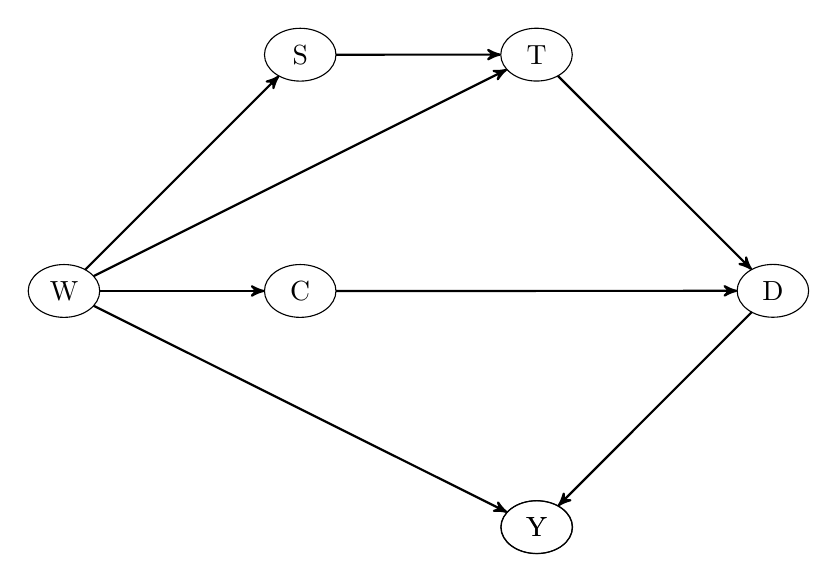
\begin{tikzpicture}[scale=1.5] 
\SetGraphUnit{2} 
\Vertex{W}  \NOEA(W){S} \EA(S){T}  \EA(W){C} \SOEA(T){D} \SOEA(C){Y} \SOWE(D){Y}
\Edges(W, S, T) \Edges(W,T) \Edges(W, C) \Edges(T, D) \Edges(C, D) \Edges(W, Y) \Edges(D, Y)
\end{tikzpicture}
\caption{Causal diagram indicating the conditional independence assumptions needed to estimate the PATT.}\label{fig:DAG}
\end{figure}

\subsection{Population Average Treatment Effect on the Treated}
The estimand of interest is 

\begin{equation}
\tau_{\text{PATT}} = \ex\left( Y_{01} - Y_{00} \mid S=0, D=1\right)
\end{equation}
This is the average treatment effect on those in the population who receive treatment.  It includes individuals who actually receive the treatment, but does not include those who are eligible for treatment and do not accept it (non-compliers).

\begin{theorem}\label{thm1}
Under assumptions \eqref{consistency} - \eqref{ER},

$$\tau_{\text{PATT}} = \ex_{01}\left[  \ex\left(Y_{11} \mid S=1, D=1, W\right)\right]
-\ex_{01}\left[  \ex\left(Y_{10} \mid S=1, T=0, C=1, W\right) \right] $$

where $\ex_{01}\left[\ex(\cdot \mid\dots, W)\right]$ denotes the expectation with respect to the distribution of $W$ in the treated individuals in the target population.  
\end{theorem}





\begin{proof}
We separate the expectation into two terms and treat each individually.
\begin{align*}
\ex\left(Y_{01} \mid S=0,D=1\right) &= \ex\left(Y_{11} \mid S=0, D=1\right) \tag*{by \eqref{consistency}} \\
&= \ex\left(Y_{11} \mid S=0, T=1, C=1\right) \tag*{by \eqref{monotonicity}} \\
&= \ex_{01}\left[  \ex\left(Y_{11} \mid S=1, T=1, C=1, W\right) \right] \tag*{by \eqref{si_treat}} \\
&= \ex_{01}\left[  \ex\left(Y_{11} \mid S=1, D=1, W\right)\right]
\end{align*}


\begin{align*}
\ex\left(Y_{00} \mid S=0, D=1\right) &= \ex\left(Y_{10} \mid S=0, D=1\right) \tag*{by \eqref{consistency}} \\
&= \ex\left(Y_{10} \mid S=0, T=1, C=1\right) \tag*{by \eqref{monotonicity}} \\
&= \ex_{01}\left[  \ex\left(Y_{10} \mid S=1, T=1, C=1, W\right) \right] \tag*{by \eqref{si_ctrl}} \\
&= \ex_{01}\left[  \ex\left(Y_{10} \mid S=1, T=0, C=1, W\right) \right] \\
\end{align*}
The last line follows because of the randomization carried out in the RCT.  This ensures $Y_{10} \independent T \mid (W, S=1)$.
\end{proof}

\subsection{Estimation Procedure}
Theorem~\ref{thm1} poses two challenges in practice.  First, we must construct an estimate of the inner expectation over potential outcomes in the RCT.  Here, we use random forests to estimate the response curve for compliers, given their treatment assignment and covariates. We estimate the outer expectation by taking empirical means.  Thus, the first term in the expression for $\tau_{\text{PATT}}$ is estimated by the weighted average of mean responses in the treatment group in the RCT. The second term is estimated by the weighted average of the mean control response for compliers assigned to control in the RCT.  We compute these by evaluating the response curve for each treated individual in the population.  \\

The second challenge is that we cannot observe which individuals are included in the estimation of the second term. We cannot tell who is a complier or non-complier in the control group, as they receive $D=0$ in either case.  We must estimate the second term by predicting who in the control group would be a complier, had they been assigned to treatment.  The exact procedure for classification isn't important, as long as predictions are made as accurate as possible. \\

The procedure for estimating $\tau_{\text{PATT}}$ using theorem~\ref{thm1} as follows:
\begin{enumerate}
\item Using the group assigned to treatment in the RCT $(S=1, T=1)$, train a model to predict complier status $C$ using the covariates $W$.
\item Using the model from step 1, predict who in the RCT assigned to control \textit{would have} complied to treatment had they been assigned to the treatment group.
\item For the group of observed compliers to treatment and predicted compliers in the control group, train a model to predict the response using as features the covariates $W$ and the treatment $T$ (assigned and observed are the same, for these individuals).  This model gives $\ex(Y_{1t} \mid S=1, C=1, T=t, W)$ for $t = 0,1$.
\item For all individuals who received treatment in the population $(S=0, D=1)$, estimate their potential outcomes $Y_{10}$ and $Y_{11}$ using the model from step 3.  The mean counterfactual $Y_{11}$ minus the mean counterfactual $Y_{10}$ is the estimate of $\tau_{\text{PATT}}$.
\end{enumerate}




\section{Simulations}
We conduct a simulation study to compare the performance of the proposed estimator, Hartman et. al's estimator, and the instrumental variables estimate of the SATE, as estimators of $\tau_{\text{PATT}}$.  Our simulation is designed so that the effect of treatment is heterogeneous and depends on other covariates, and the design satisfies the conditional independence assumptions in Figure~\ref{fig:DAG}.

\subsection{Simulation Design}
RCT eligibility, complier status, and treatment assignment in the population depend on observed covariates. 
The observed covariates $(W_1, W_2, W_3)$ are multivariate normal with mean $(0.5, 1, -1)$ and covariances $\cov(W_1, W_2) = 1$ and $\cov(W_1, W_3) = \cov(W_2, W_3) = 0.5$. 
 The  equation for selection into studies is
 $$ S = \ind(e_2 + g_1W_1 + g_2W_2 + g_3W_3 + R > 0)$$
  where $R$ is standard normal. $e_2$ controls the fraction of the population eligible for the RCT. We set $g_1, g_2,$ and $g_3$ to be $0.5,$ $0.25,$ and $0.75$, respectively.
Complier status is determined by
$$C = \ind(e_3 + h_2W_2 + h_3W_3 + Q > 0)$$
where $Q$ is standard normal. $e_3$ controls the fraction of compliers in the population. We set $h_2$ and $h_3$ to $0.5$.
 For individuals in the population ($S=0$),  treatment is assigned by
  $$T = \ind(e_1 + f_1W_1 + f_2W_2 + V > 0)$$
Varying $e_1$ controls the fraction eligible for treatment in the population. $V$ is standard normal. We set $f_1$ to $0.25$ and $f_2$ to $0.75$.  For individuals in the RCT ($S=1$), treatment assignment is a sample from a Bernoulli distribution.
We set treatment received $D$ according to $T$ and $C$: $D = T$ if $C=1$ and $D = 0$ if $C=0$.
Finally, the response $Y$ is determined by 
$$Y = a + bD + c_1W_1 + c_2W_2 + dU$$
 We assume that the treatment effect $b$ is heterogeneous depending on $W_1$: $b = 1$ if $W_1 > 0.75$ and $b=-1$ if $W_1 \leq 0.75$.   We set $a, c_1,$ and $d$ to $1$ and $c_2$ to $2$. $U$ is standard normal and $U, V, R, Q, (W_1, W_2, W_3)$ are mutually independent.\\
 
 We generate a population of 30,000 individuals and randomly sample 5,000.  Those among the 5,000 who are eligible for the RCT ($S=1$) are selected. Similarly, we sample 5,000 individuals from the population and select those who are not eligible for the RCT ($S=0$); these are a sample of the ``target population''.  We set each individual's treatment received $D$ according to their treatment assignment and complier status and observe their responses $Y$.  In this design, the way that we've set $S, T, D, C,$ and $Y$ ensures that assumptions \eqref{consistency} - \eqref{ER} hold.\\
 
In the assigned-treatment RCT group $(S = 1, T = 1)$, we fit a logistic regression to compliance status using the covariates.  With this model, we predict who in the control group $(S = 1, T = 0)$ has $C=1$, since this is unobservable.  These individuals \textit{would have} complied had they been assigned to the treatment group.  For this group of observed compliers to treatment and predicted compliers from the control group of the RCT, we estimate the response curve using a random forest with features $(W_1, W_2, W_3)$ and $D$.  Then population local average treatment effect on the treated is estimated according to the estimation procedure outlined above.


\subsection{Simulation results}

We vary each of the parameters $e_1, e_2,$ and $e_3$ along a grid by $-2$ to $2$ in increments of $0.5$ in order to generate different combinations of rates of compliance, treatment eligibility, and RCT eligibility in the population of 30,000.  For each possible combination of the three parameters, we run the simulation $5$ times and compute the mean squared error of our proposed estimator for $\tau_{\text{PATT}}$ that adjusts for non-compliance, the estimator from Hartman et. al which is unadjusted for non-compliance, and the SATE using the instrumental variables estimator from \cite{Angrist1996}, given by the intention-to-treat estimate divided by the rate of compliance.  All other parameters are held fixed. The unadjusted estimate is obtained by estimating the response curve on all individuals in the RCT and applying step 4 of our proposed estimation procedure to the non-randomized trial individuals. \\

Figure~\ref{fig:sim_tiles} shows the relationship between the percent of compliers in the whole population, the percentage of people in the whole population eligible to participate in the RCT, and the mean squared error of the PATT estimators.  The pattern of performance is qualitatively similar for the adjusted and unadjusted estimators: both perform best when compliance is high and perform badly when compliance is low.  Furthermore, for a fixed rate of compliance, the estimators tend to have lower mean squared error when either a very small or very large fraction of the total population is eligible to participate in the RCT. \\



\begin{figure}[htbp]
\begin{center}
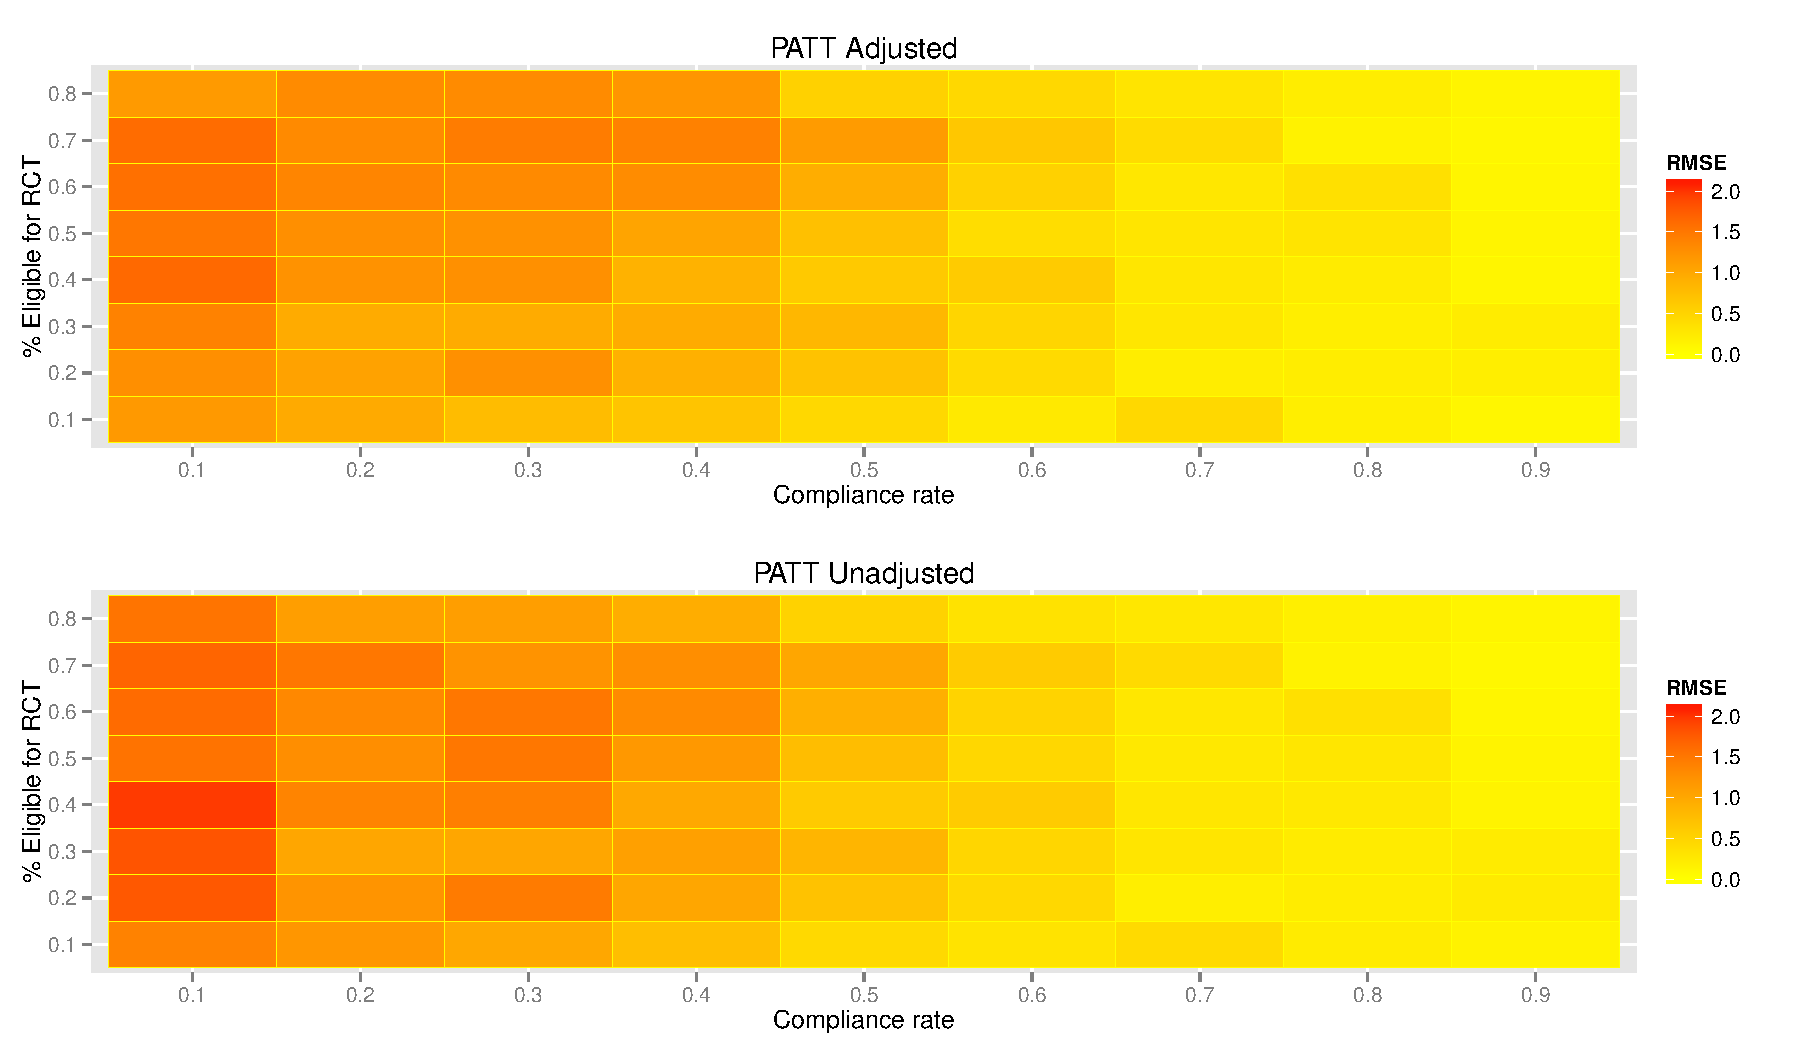
\includegraphics[width = 0.8\textwidth]{mse_ratec_rates_B5}
\caption{Simulation mean squared error, transformed by -$\log$. Darker tiles correspond to lower mean squared error.}
\label{fig:sim_tiles}
\end{center}
\end{figure}

Figure~\ref{fig:sim_compliance} compares the mean squared error of the two PATT estimators and the SATE (as an estimator of PATT) at varying levels of compliance in the total population.  When compliance is low, both PATT estimators have a large mean squared error and variance.  The adjusted estimator has a large variance because the subset of the RCT who are considered compliers is relatively small, whereas the unadjusted estimator has large variance because of the large amount of crossover.  For low levels of compliance, SATE actually tends to approximate PATT more closely; the variance due to small sample size is contributes less to the mean squared error than the bias due to crossover in the other two estimators.  On the other hand, when the compliance rate is high, both PATT estimators perform about equally well with mean squared error close to $0$.  Meanwhile, he median mean squared error for SATE stays relatively constant regardless of compliance rate.  This shows that the instrumental variables estimate of SATE is able to adjust for the non-compliance, but is unable to account for differences in pretreatment covariates between the RCT sample and target population.

\begin{figure}[htbp]
\begin{center}
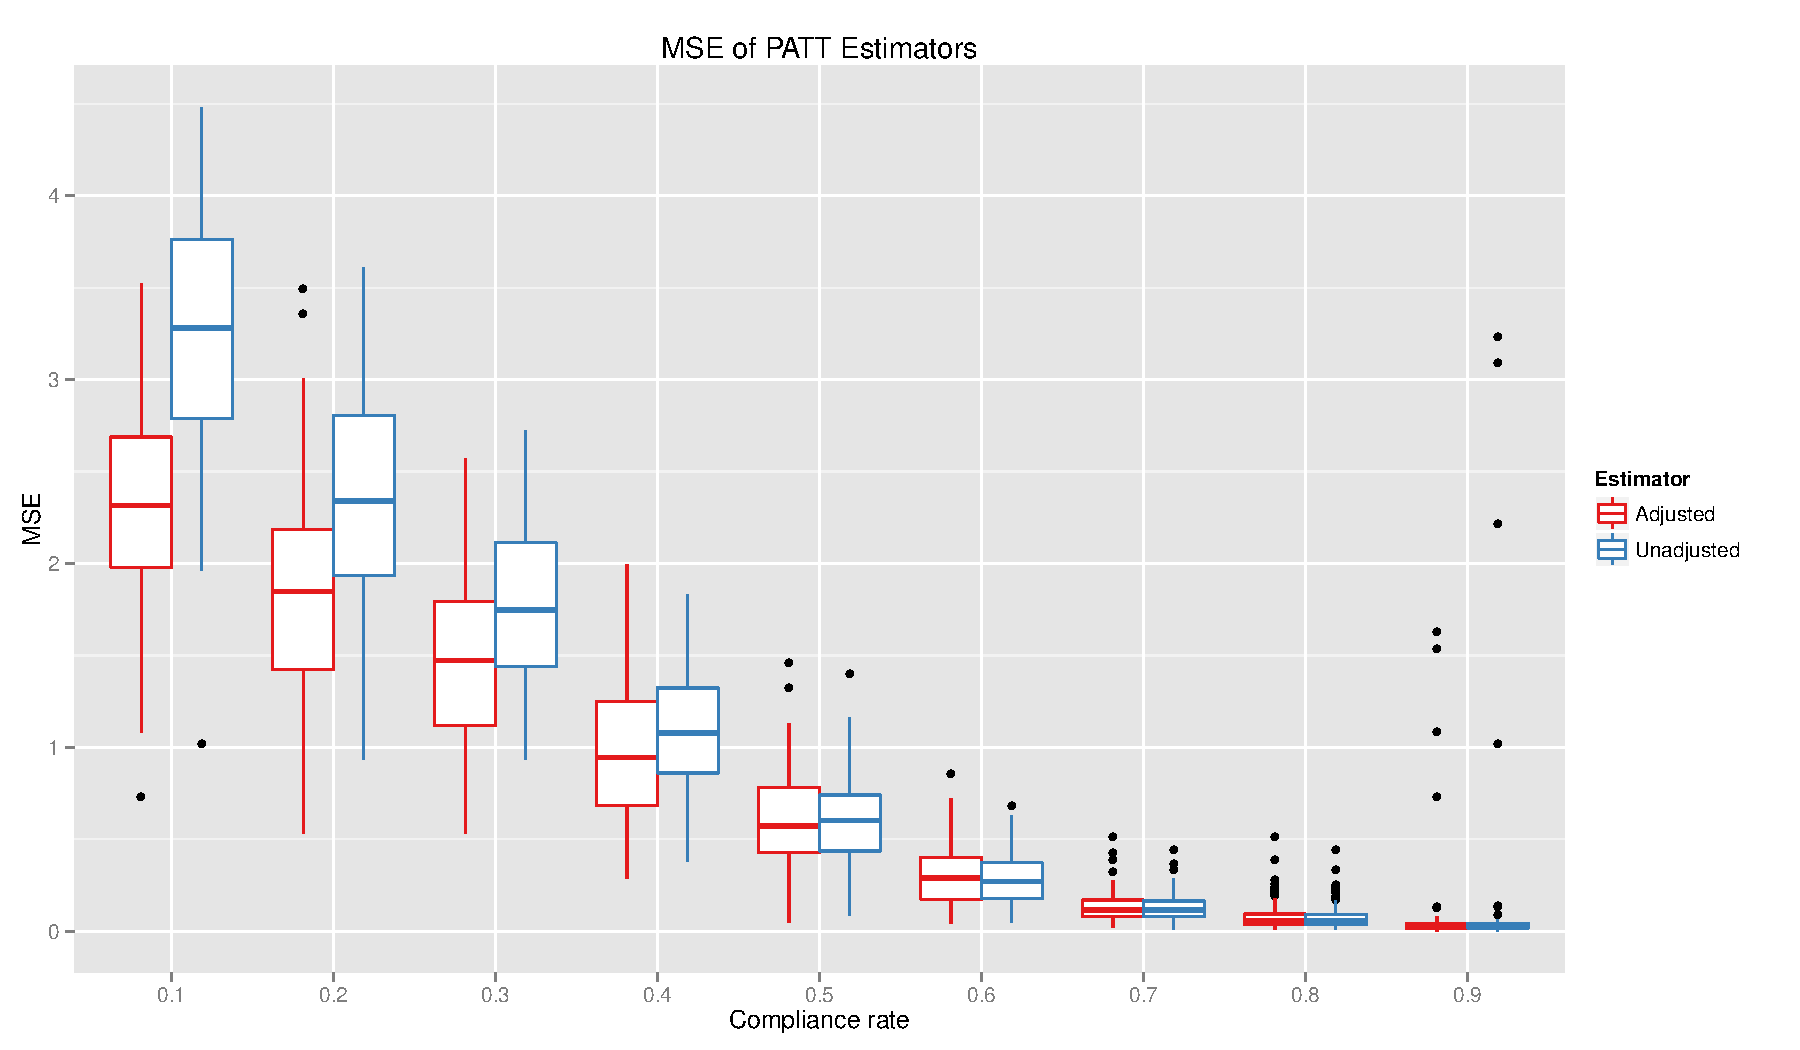
\includegraphics[width = 0.8\textwidth]{mse_boxplots_B5}
\caption{Simulation mean squared error, according to compliance rates in the total population.}
\label{fig:sim_compliance}
\end{center}
\end{figure}





\section{Empirical Example: Medicaid and Hospital Use}
\subsection{Data}

We apply the proposed method to estimate the effect of extending Medicaid coverage on health care use.  Medicaid is a federally-funded program, so understanding how the RCT estimates generalize to a broader population of individuals who will be covered by other Medicaid expansions is informative for public policy. In particular, we examine the population of nonelderly adults in the U.S. with household incomes at or below 138\% of the FPL (\$32,913 for a four--person household in 2014) who may be eligible for Medicaid following the Affordable Care Act (ACA) expansion.

\paragraph{Oregon Health Insurance Experiment}

We draw RCT data from the Oregon Health Insurance Experiment (OHIE) \cite{finkelstein2012,Taubman}.  In 2008, approximately 90,000 uninsured low-income adults participated in a lottery to receive Medicaid benefits.\footnote{Eligible participants include Oregon residents (US citizens or legal immigrants) aged 19 to 64 not otherwise eligible for public insurance, who who have been without insurance for six months, and have income below the FPL and assets below \$2,000.} Treatment occurred at the household level: participants selected by the lottery won the opportunity for themselves and any household member to apply for Medicaid. Sample exclusions brought the sample size down to 74,922 individuals representing 66,385 households.  Within the sample, 29,834 participants were selected by the lottery; the remaining 45,008 participants served as controls in the experiment.  Participants in selected households received benefits if they returned an enrollment application within 45 days of receipt. Among participants in selected households, about 60\% mailed back applications and only 30\% successfully enrolled.\footnote{About half of the returned applications were deemed ineligible, primarily due to failure to demonstrate income below the FPL. Enrolled participants were required to recertify their eligibility status every six months.} We use the following pretreatment covariates as features in our prediction models: gender, age, race, ethnicity, health status, education, and household income.\footnote{Since randomization is applied on the household level, we include the number of household members as a feature in all prediction models. Treatment is included as a feature in the response models.}  \\

We use two health care use responses: emergency room (ER) and primary care visits in the past 12 months.\footnote{The variables that capture the total number of visits have been censored so that no individual value has fewer than ten observations.} These data originate from a mail survey that was administered to participants over July and August 2009 ($N = 23,741$ survey respondents) \cite{finkelstein2012}. We use the same definition of insurance coverage as \citet{finkelstein2012} to form our measure of compliance, which is a binary variable indicating whether the participant was enrolled in any Medicaid program (including the lotteried program) between the notification date and 30 September 2009. While \possessivecite{finkelstein2012} IVLS estimates of the effect of Medicaid assume one--way crossover, 14\% of control participants were actually enrolled in Medicaid during the study period (compared to the 60\% of treated participants who did not enroll). 

\paragraph{Observational data} 

We employ data on the target population from the National Health Interview Study (NHIS) \cite{NHIS}, which is conducted by the Center for Disease Control.  We restrict our analysis to respondents whose income is below 138\% of the FPL. We use covariates on respondent characteristics that match the OHIE pretreatment covariates. The outcomes of interest from NHIS are variables on ER  and primary care visits in the past 12 months. We use a recoded variable which indicates whether respondents are on Medicaid as an analogue to the OHIE compliance measure.

\subsection{Verifying assumptions}

Are the assumptions stated in Section \ref{estimator} satisfied by the data? Assumption \eqref{consistency} ensures that potential outcomes for participants in the target population (i.e., respondents in the NHIS sample) would be identical to their outcomes in the RCT if they had been randomly assigned their observed treatment. A violation of the consistency assumption might arise, for instance, if there are differences in the mail surveys used to illicit health care use responses.

\todo{Discuss how the assumptions for estimating PATT are met or not met by the data -- just brainstorming for now}
\begin{enumerate}
\item Consistency under parallel studies
\item Strong ignorability of sample assignment for treated
\item Strong ignorability of sample assignment for controls
\item SUTVA
\item Conditional independence of compliance and treatment assignment
\item Monotonicity: not satisfied! how did we address this?
\item Exclusion restriction: It would seem reasonable that whether or not someone actually has Medicaid, not their eligibility to enroll, would affect their hospital use.  For generic health insurance one might argue that eligibility could be negatively correlated with hospital use, as people with pre-existing conditions may be less likely to be eligible yet go to the hospital more frequently.  This should not be the case with a federally funded program such as Medicaid.
\end{enumerate}


\subsection{Empirical results}

\begin{figure}
\begin{center}
  \begin{subfigure}[b]{0.86\textwidth}
    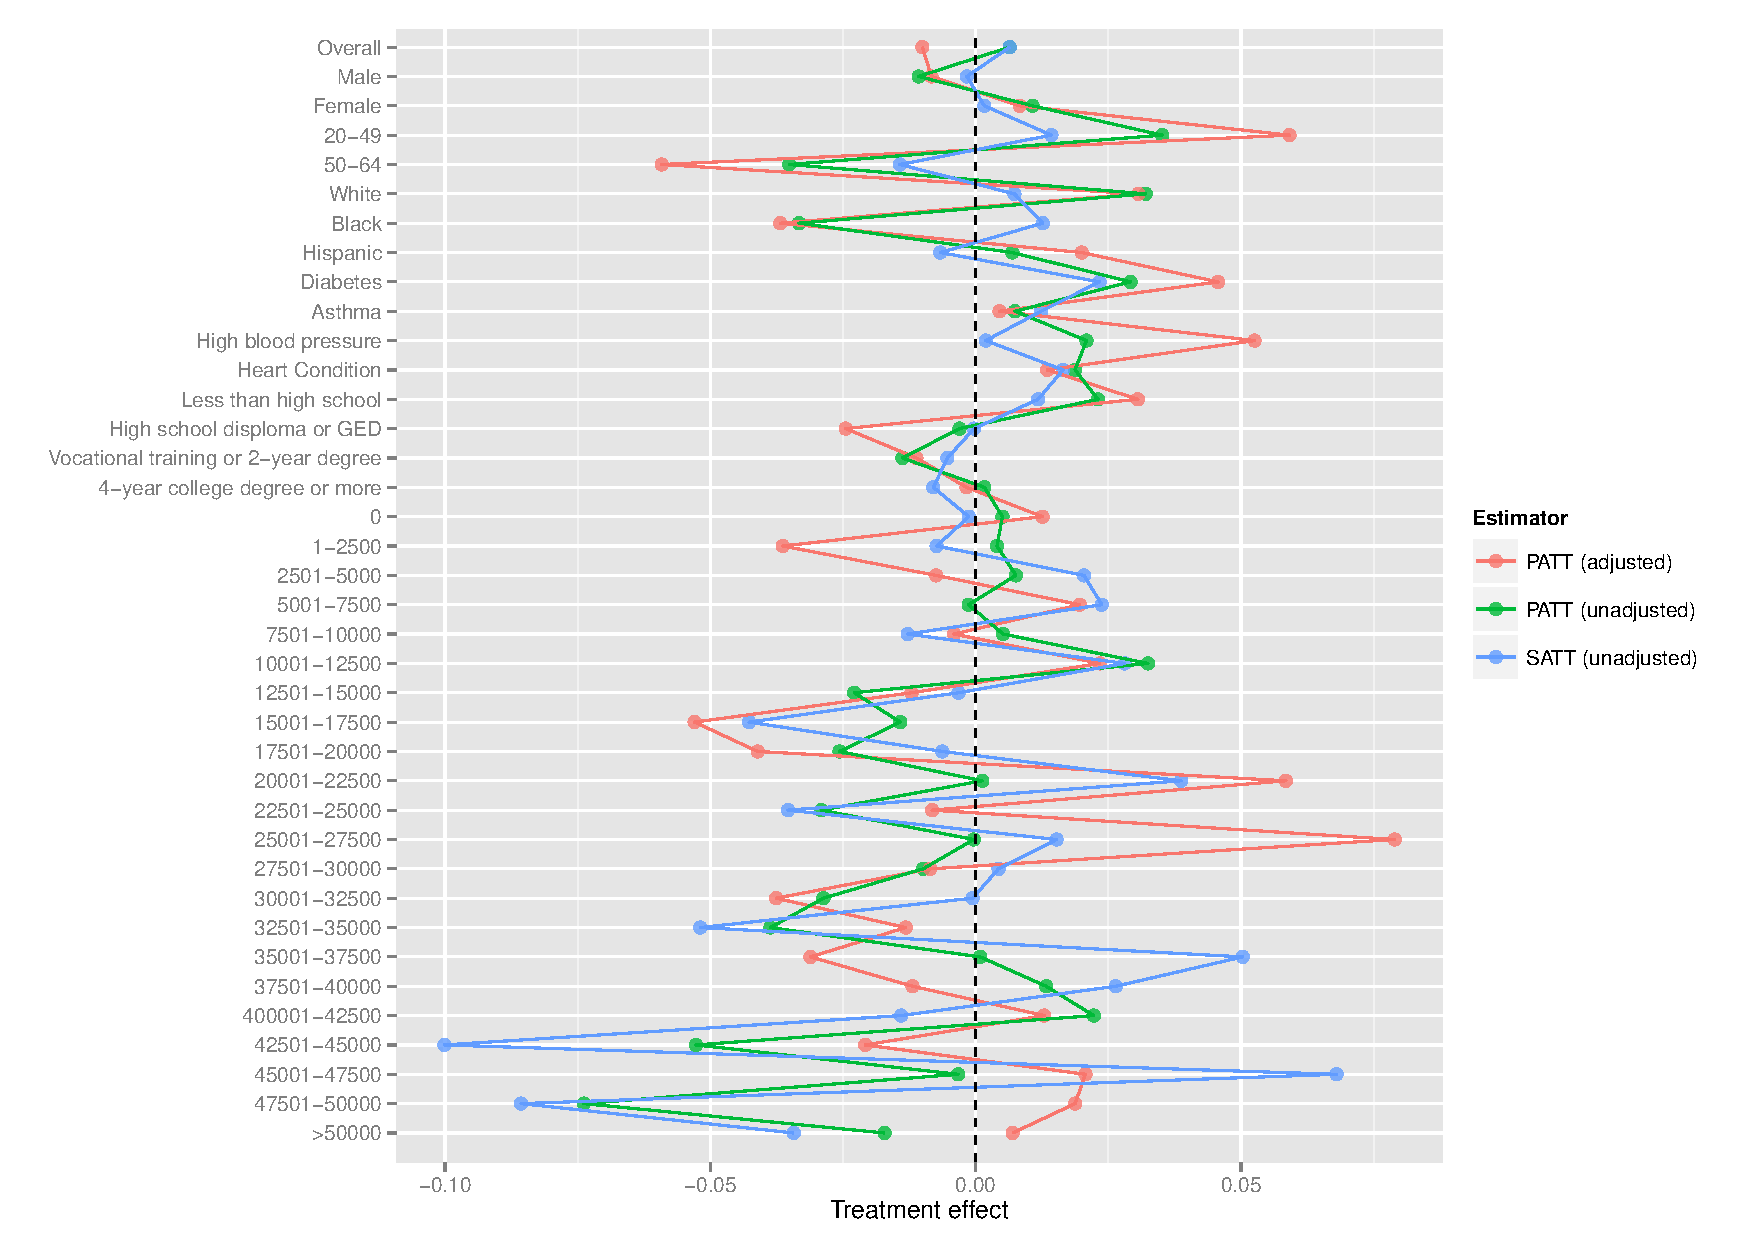
\includegraphics[width=\textwidth]{any-visit-plot.pdf}
    \caption{Any ER visit.}
    \label{fig:any-visit-plot}
  \end{subfigure}
  %
  \begin{subfigure}[b]{0.86\textwidth}
    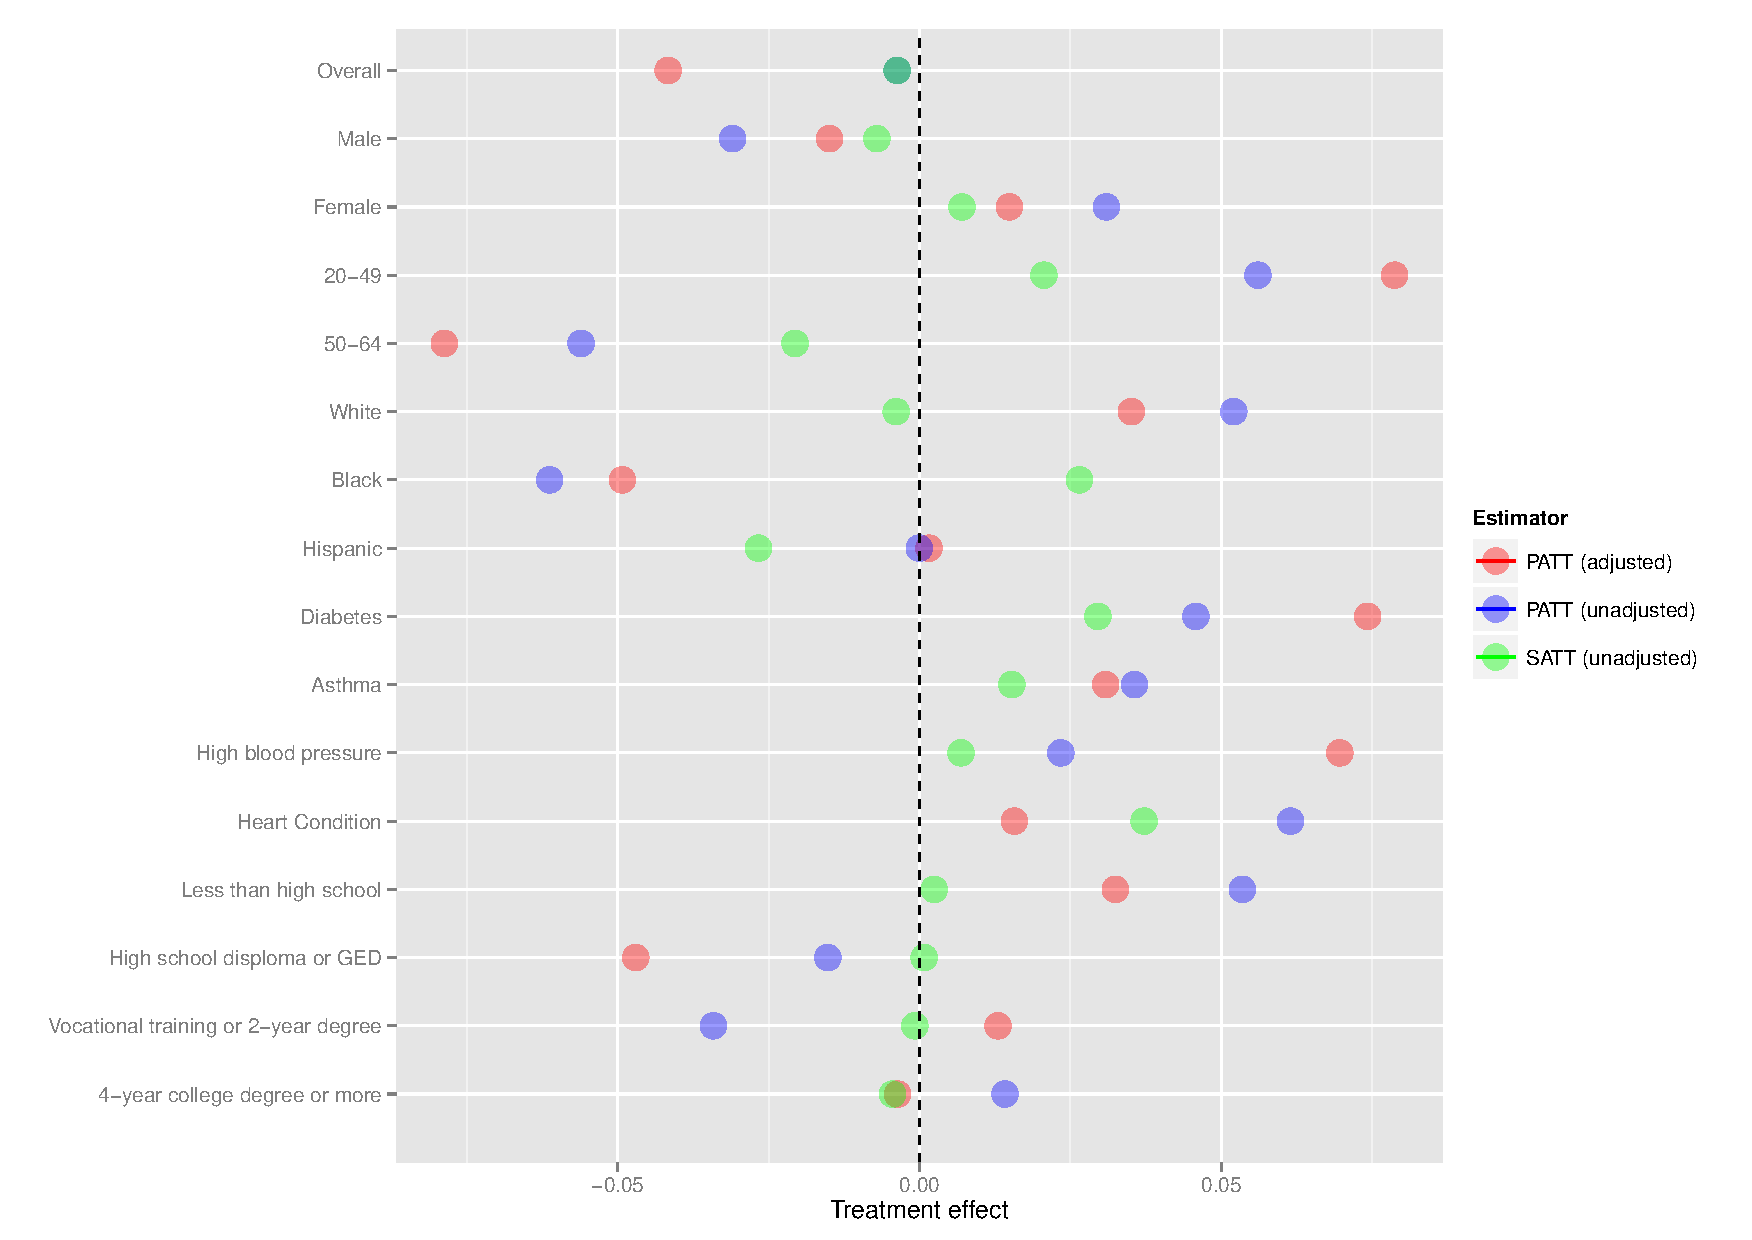
\includegraphics[width=\textwidth]{num-visit-plot.pdf}
    \caption{Number of ER visits.}
    \label{fig:num-visit-plot}
  \end{subfigure}
 \caption{Comparison of estimators for treatment effect on ER use.}
  \end{center}
 \label{fig:ER-visit}
\end{figure}

\begin{figure}
\begin{center}
     \begin{subfigure}[b]{0.86\textwidth}
    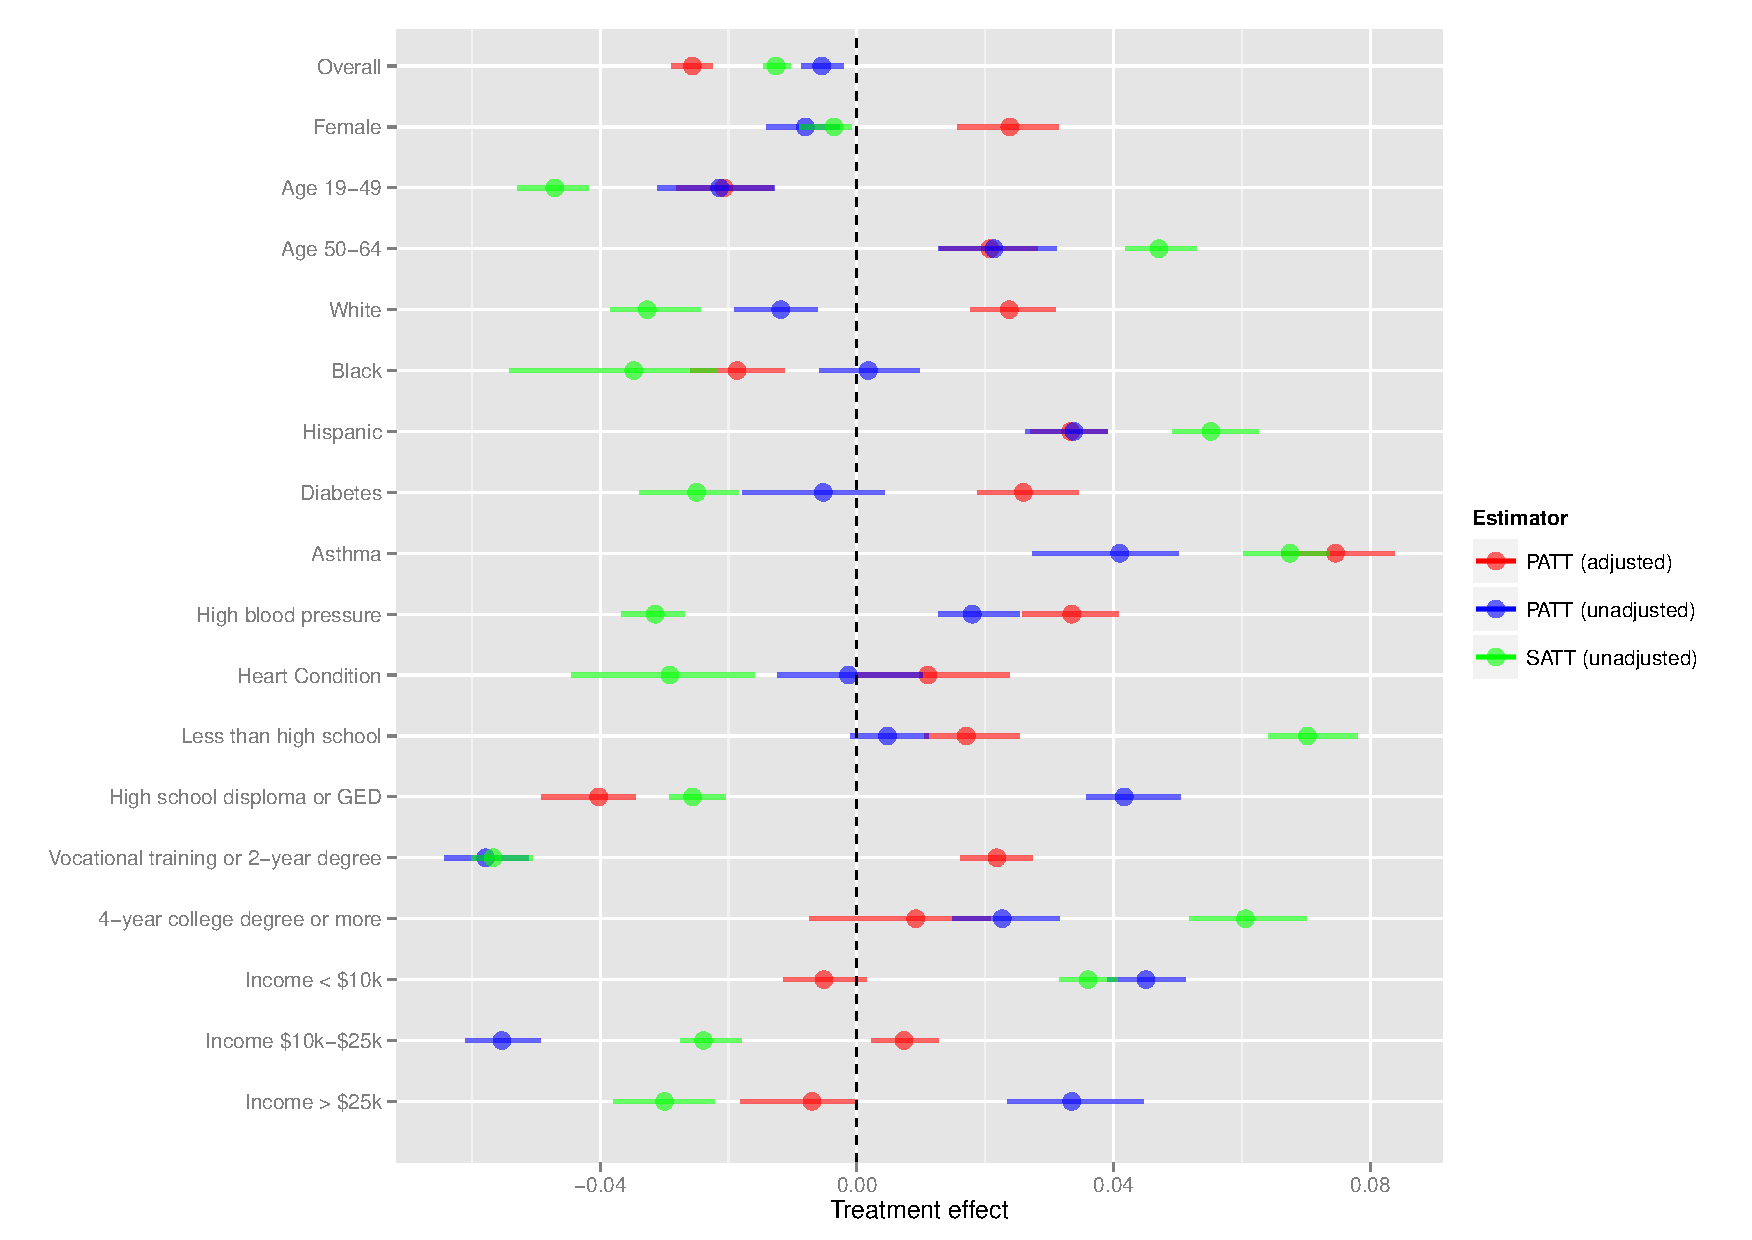
\includegraphics[width=\textwidth]{any-out-plot.pdf}
    \caption{Any primary care visit.}
    \label{fig:any-out-plot}
  \end{subfigure}
    %
    \begin{subfigure}[b]{0.86\textwidth}
    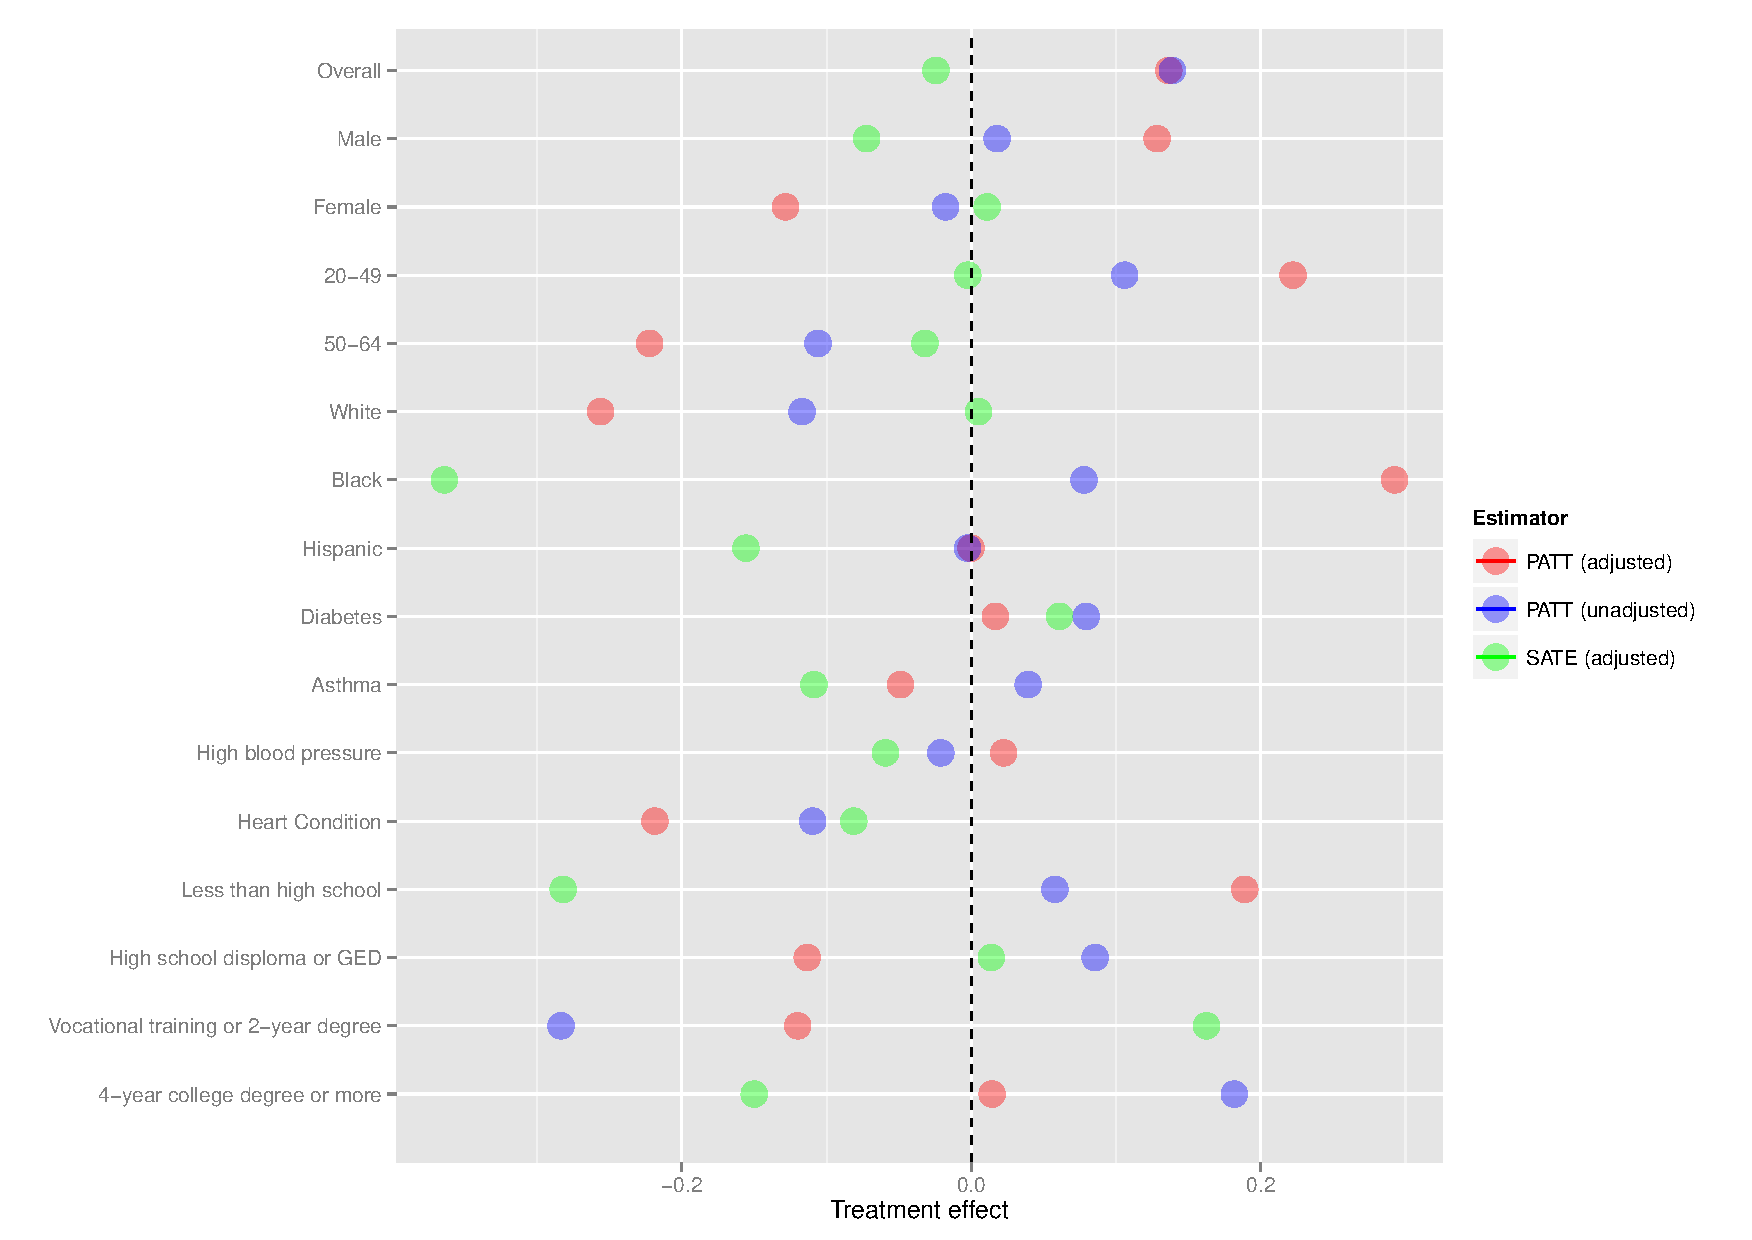
\includegraphics[width=\textwidth]{num-out-plot.pdf}
    \caption{Number of primary care visits.}
    \label{fig:num-out-plot}
  \end{subfigure}
  \caption{Comparison of estimators for treatment effect on primary care use.}
   \end{center}
   \label{fig:out-visit}
\end{figure}

% Compare with table A28 of F2012
\section{Discussion}

The treatment effect of Medicaid applies to uninsured adults with income below the FPL who express interest in health insurance coverage. The sample population differs in several dimensions from the target population of individuals who will be covered by other Medicaid expansions, such as the ACA expansion to cover all adults up to 138\% of the FPL. For instance, the RCT participants are disproportionately white urban--dwellers \cite{Taubman}. The RCT participants volunteered for the study and therefore may be in poorer health compared to the population. \\

Simulations shed light on the conditions under which the proposed estimator should work well.  When the rate of crossover from treatment to control is low, the proposed estimator performs better than the estimator which doesn't adjust for non-compliance.  Here, the unadjusted estimator gives the intention-to-treat effect, which tends to underestimate the average treatment effect on compliers. Of course, the simulation results depend on the particular way we parameterized the compliance, selection, treatment assignment, and response schedules.  In particular, the strength of correlation between the covariates and compliance governs how well the estimator will perform, since step one of the estimation procedure is to predict who \textit{would be} a complier in the RCT control group, had they been assigned to treatment. If it is difficult to predict compliance using the observed covariates, then the estimator will perform badly because of noise introduced by incorrectly treating non-compliers as compliers.  Further research should be done into ways to test how well compliance can be predicted. \\

In the OHIE trial, only about $30\%$ of those selected to receive Medicaid benefits actually enrolled successfully, and successful enrollment depended in part on income levels.  The proposed estimator that adjusts for non-compliance seems to perform better than the unadjusted estimator when compliance is low and can be predicted by observed covariates (Figure~\ref{fig:sim_compliance}).  Our random forest for predicting compliance based on observed covariates has about $61.5\%$ accuracy on the training set of individuals in OHIE assigned to the treatment group.  While we don't know well how the model predicts for the control group, its performance on the training set suggests that compliance is not purely random, but depends on observed covariates.  This gives evidence in favor of using the proposed estimator.  Future work should be done to construct a better model to predict compliance, both in the treated group used for training and the controls in the RCT. \\


\todo{Update to reflect what we expected + what we actually saw}
The proposed method allows us to decompose both SATE and PATT estimates by subgroup according to covariates common to both RCT and observational datasets (e.g, demographic variables, pre--existing conditions, and insurance coverage). Since the RCT participants are predominately white and volunteered for the study, we expect to find substantial differences between sample and population estimates in terms of ethnicity and pre--existing condition subgroups. Overall, we expect the PATT estimate to be lower than the SATE estimate due to the adverse selection problem in the RCT. \\




\pagebreak

\begin{singlespace}		%Single-space for bibliography 

%Bibliography
\bibliographystyle{plainnat}
\bibliography{refs}

%Appendix
\pagebreak
\begin{appendices}

\end{appendices}
\end{singlespace}

\itemize
\end{document}


